\documentclass{ximera}

%\usepackage{todonotes}

\newcommand{\todo}{}

\usepackage{esint} % for \oiint
\ifxake%%https://math.meta.stackexchange.com/questions/9973/how-do-you-render-a-closed-surface-double-integral
\renewcommand{\oiint}{{\large\bigcirc}\kern-1.56em\iint}
\fi


\graphicspath{
  {./}
  {ximeraTutorial/}
  {basicPhilosophy/}
  {functionsOfSeveralVariables/}
  {normalVectors/}
  {lagrangeMultipliers/}
  {vectorFields/}
  {greensTheorem/}
  {shapeOfThingsToCome/}
  {dotProducts/}
  {partialDerivativesAndTheGradientVector/}
  {../productAndQuotientRules/exercises/}
  {../normalVectors/exercisesParametricPlots/}
  {../continuityOfFunctionsOfSeveralVariables/exercises/}
  {../partialDerivativesAndTheGradientVector/exercises/}
  {../directionalDerivativeAndChainRule/exercises/}
  {../commonCoordinates/exercisesCylindricalCoordinates/}
  {../commonCoordinates/exercisesSphericalCoordinates/}
  {../greensTheorem/exercisesCurlAndLineIntegrals/}
  {../greensTheorem/exercisesDivergenceAndLineIntegrals/}
  {../shapeOfThingsToCome/exercisesDivergenceTheorem/}
  {../greensTheorem/}
  {../shapeOfThingsToCome/}
  {../separableDifferentialEquations/exercises/}
  {vectorFields/}
}

\newcommand{\mooculus}{\textsf{\textbf{MOOC}\textnormal{\textsf{ULUS}}}}

\usepackage{tkz-euclide}
\usepackage{tikz}
\usepackage{tikz-cd}
\usetikzlibrary{arrows}
\tikzset{>=stealth,commutative diagrams/.cd,
  arrow style=tikz,diagrams={>=stealth}} %% cool arrow head
\tikzset{shorten <>/.style={ shorten >=#1, shorten <=#1 } } %% allows shorter vectors

\usetikzlibrary{backgrounds} %% for boxes around graphs
\usetikzlibrary{shapes,positioning}  %% Clouds and stars
\usetikzlibrary{matrix} %% for matrix
\usepgfplotslibrary{polar} %% for polar plots
\usepgfplotslibrary{fillbetween} %% to shade area between curves in TikZ
%\usetkzobj{all}
\usepackage[makeroom]{cancel} %% for strike outs
%\usepackage{mathtools} %% for pretty underbrace % Breaks Ximera
%\usepackage{multicol}
\usepackage{pgffor} %% required for integral for loops



%% http://tex.stackexchange.com/questions/66490/drawing-a-tikz-arc-specifying-the-center
%% Draws beach ball
\tikzset{pics/carc/.style args={#1:#2:#3}{code={\draw[pic actions] (#1:#3) arc(#1:#2:#3);}}}



\usepackage{array}
\setlength{\extrarowheight}{+.1cm}
\newdimen\digitwidth
\settowidth\digitwidth{9}
\def\divrule#1#2{
\noalign{\moveright#1\digitwidth
\vbox{\hrule width#2\digitwidth}}}




% \newcommand{\RR}{\mathbb R}
% \newcommand{\R}{\mathbb R}
% \newcommand{\N}{\mathbb N}
% \newcommand{\Z}{\mathbb Z}

\newcommand{\sagemath}{\textsf{SageMath}}


%\renewcommand{\d}{\,d\!}
%\renewcommand{\d}{\mathop{}\!d}
%\newcommand{\dd}[2][]{\frac{\d #1}{\d #2}}
%\newcommand{\pp}[2][]{\frac{\partial #1}{\partial #2}}
% \renewcommand{\l}{\ell}
%\newcommand{\ddx}{\frac{d}{\d x}}

% \newcommand{\zeroOverZero}{\ensuremath{\boldsymbol{\tfrac{0}{0}}}}
%\newcommand{\inftyOverInfty}{\ensuremath{\boldsymbol{\tfrac{\infty}{\infty}}}}
%\newcommand{\zeroOverInfty}{\ensuremath{\boldsymbol{\tfrac{0}{\infty}}}}
%\newcommand{\zeroTimesInfty}{\ensuremath{\small\boldsymbol{0\cdot \infty}}}
%\newcommand{\inftyMinusInfty}{\ensuremath{\small\boldsymbol{\infty - \infty}}}
%\newcommand{\oneToInfty}{\ensuremath{\boldsymbol{1^\infty}}}
%\newcommand{\zeroToZero}{\ensuremath{\boldsymbol{0^0}}}
%\newcommand{\inftyToZero}{\ensuremath{\boldsymbol{\infty^0}}}



% \newcommand{\numOverZero}{\ensuremath{\boldsymbol{\tfrac{\#}{0}}}}
% \newcommand{\dfn}{\textbf}
% \newcommand{\unit}{\,\mathrm}
% \newcommand{\unit}{\mathop{}\!\mathrm}
% \newcommand{\eval}[1]{\bigg[ #1 \bigg]}
% \newcommand{\seq}[1]{\left( #1 \right)}
% \renewcommand{\epsilon}{\varepsilon}
% \renewcommand{\phi}{\varphi}


% \renewcommand{\iff}{\Leftrightarrow}

% \DeclareMathOperator{\arccot}{arccot}
% \DeclareMathOperator{\arcsec}{arcsec}
% \DeclareMathOperator{\arccsc}{arccsc}
% \DeclareMathOperator{\si}{Si}
% \DeclareMathOperator{\scal}{scal}
% \DeclareMathOperator{\sign}{sign}


%% \newcommand{\tightoverset}[2]{% for arrow vec
%%   \mathop{#2}\limits^{\vbox to -.5ex{\kern-0.75ex\hbox{$#1$}\vss}}}
% \newcommand{\arrowvec}[1]{{\overset{\rightharpoonup}{#1}}}
% \renewcommand{\vec}[1]{\arrowvec{\mathbf{#1}}}
% \renewcommand{\vec}[1]{{\overset{\boldsymbol{\rightharpoonup}}{\mathbf{#1}}}}

% \newcommand{\point}[1]{\left(#1\right)} %this allows \vector{ to be changed to \vector{ with a quick find and replace
% \newcommand{\pt}[1]{\mathbf{#1}} %this allows \vec{ to be changed to \vec{ with a quick find and replace
% \newcommand{\Lim}[2]{\lim_{\point{#1} \to \point{#2}}} %Bart, I changed this to point since I want to use it.  It runs through both of the exercise and exerciseE files in limits section, which is why it was in each document to start with.

% \DeclareMathOperator{\proj}{\mathbf{proj}}
% \newcommand{\veci}{{\boldsymbol{\hat{\imath}}}}
% \newcommand{\vecj}{{\boldsymbol{\hat{\jmath}}}}
% \newcommand{\veck}{{\boldsymbol{\hat{k}}}}
% \newcommand{\vecl}{\vec{\boldsymbol{\l}}}
% \newcommand{\uvec}[1]{\mathbf{\hat{#1}}}
% \newcommand{\utan}{\mathbf{\hat{t}}}
% \newcommand{\unormal}{\mathbf{\hat{n}}}
% \newcommand{\ubinormal}{\mathbf{\hat{b}}}

% \newcommand{\dotp}{\bullet}
% \newcommand{\cross}{\boldsymbol\times}
% \newcommand{\grad}{\boldsymbol\nabla}
% \newcommand{\divergence}{\grad\dotp}
% \newcommand{\curl}{\grad\cross}
%\DeclareMathOperator{\divergence}{divergence}
%\DeclareMathOperator{\curl}[1]{\grad\cross #1}
% \newcommand{\lto}{\mathop{\longrightarrow\,}\limits}

% \renewcommand{\bar}{\overline}

\colorlet{textColor}{black}
\colorlet{background}{white}
\colorlet{penColor}{blue!50!black} % Color of a curve in a plot
\colorlet{penColor2}{red!50!black}% Color of a curve in a plot
\colorlet{penColor3}{red!50!blue} % Color of a curve in a plot
\colorlet{penColor4}{green!50!black} % Color of a curve in a plot
\colorlet{penColor5}{orange!80!black} % Color of a curve in a plot
\colorlet{penColor6}{yellow!70!black} % Color of a curve in a plot
\colorlet{fill1}{penColor!20} % Color of fill in a plot
\colorlet{fill2}{penColor2!20} % Color of fill in a plot
\colorlet{fillp}{fill1} % Color of positive area
\colorlet{filln}{penColor2!20} % Color of negative area
\colorlet{fill3}{penColor3!20} % Fill
\colorlet{fill4}{penColor4!20} % Fill
\colorlet{fill5}{penColor5!20} % Fill
\colorlet{gridColor}{gray!50} % Color of grid in a plot

\newcommand{\surfaceColor}{violet}
\newcommand{\surfaceColorTwo}{redyellow}
\newcommand{\sliceColor}{greenyellow}




\pgfmathdeclarefunction{gauss}{2}{% gives gaussian
  \pgfmathparse{1/(#2*sqrt(2*pi))*exp(-((x-#1)^2)/(2*#2^2))}%
}


%%%%%%%%%%%%%
%% Vectors
%%%%%%%%%%%%%

%% Simple horiz vectors
\renewcommand{\vector}[1]{\left\langle #1\right\rangle}


%% %% Complex Horiz Vectors with angle brackets
%% \makeatletter
%% \renewcommand{\vector}[2][ , ]{\left\langle%
%%   \def\nextitem{\def\nextitem{#1}}%
%%   \@for \el:=#2\do{\nextitem\el}\right\rangle%
%% }
%% \makeatother

%% %% Vertical Vectors
%% \def\vector#1{\begin{bmatrix}\vecListA#1,,\end{bmatrix}}
%% \def\vecListA#1,{\if,#1,\else #1\cr \expandafter \vecListA \fi}

%%%%%%%%%%%%%
%% End of vectors
%%%%%%%%%%%%%

%\newcommand{\fullwidth}{}
%\newcommand{\normalwidth}{}



%% makes a snazzy t-chart for evaluating functions
%\newenvironment{tchart}{\rowcolors{2}{}{background!90!textColor}\array}{\endarray}

%%This is to help with formatting on future title pages.
\newenvironment{sectionOutcomes}{}{}



%% Flowchart stuff
%\tikzstyle{startstop} = [rectangle, rounded corners, minimum width=3cm, minimum height=1cm,text centered, draw=black]
%\tikzstyle{question} = [rectangle, minimum width=3cm, minimum height=1cm, text centered, draw=black]
%\tikzstyle{decision} = [trapezium, trapezium left angle=70, trapezium right angle=110, minimum width=3cm, minimum height=1cm, text centered, draw=black]
%\tikzstyle{question} = [rectangle, rounded corners, minimum width=3cm, minimum height=1cm,text centered, draw=black]
%\tikzstyle{process} = [rectangle, minimum width=3cm, minimum height=1cm, text centered, draw=black]
%\tikzstyle{decision} = [trapezium, trapezium left angle=70, trapezium right angle=110, minimum width=3cm, minimum height=1cm, text centered, draw=black]


\title{Parabolas}

\begin{document}

\begin{abstract}
quadratic graphs
\end{abstract}
\maketitle





We have three forms for quadratic functions (or equations):



$\blacktriangleright$ $S(x) = A \, x^2 + B \, x + C$  with $A \ne 0$ : Standard Form. \\


$\blacktriangleright$ $F(t) = A \, (t - r_1)(t - r_2)$  with $A \ne 0$ : Factored Form. \\


$\blacktriangleright$ $V(d) = A \, (d - h)^2 + k$  with $A \ne 0$ : Vertex Form. \\




Vertex form comes from completing the square.  It gets its name from the graph of quadratic functions.









\subsection*{Graphs of Quadratic Functions}



Quadratic functions all have parabolas for graphs.




\begin{image}
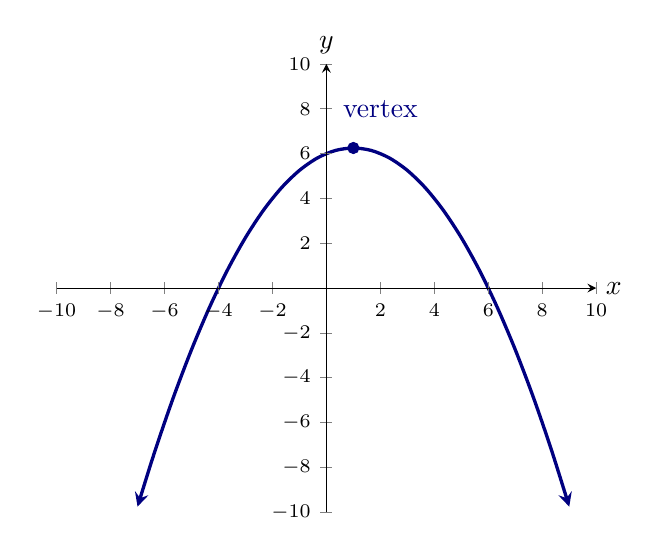
\begin{tikzpicture}
     \begin{axis}[
                domain=-10:10, ymax=10, xmax=10, ymin=-10, xmin=-10,
                axis lines =center, xlabel=$x$, ylabel=$y$,
                ytick={-10,-8,-6,-4,-2,2,4,6,8,10},
            	xtick={-10,-8,-6,-4,-2,2,4,6,8,10},
            	ticklabel style={font=\scriptsize},
                every axis y label/.style={at=(current axis.above origin),anchor=south},
                every axis x label/.style={at=(current axis.right of origin),anchor=west},
                axis on top,
                ]



        \addplot [draw=penColor, very thick, smooth, domain=(-7:9),<->] {-0.25*(x+4)*(x-6)};
        %\addplot [line width=1, gray, dashed,samples=100,domain=(-9.5:9.5)] ({3},{x});
        


        \addplot [color=penColor,only marks,mark=*] coordinates{(1,6.25)};
        \node[penColor] at (axis cs:2,8) {vertex};
        %\node[penColor] at (axis cs:4,1.5) {$(h, k)$};
        %\node[penColor] at (axis cs:5,-9) {$-0.5 x^2 - 5 x + 15.5$};



    \end{axis}
\end{tikzpicture}
\end{image}











\begin{image}
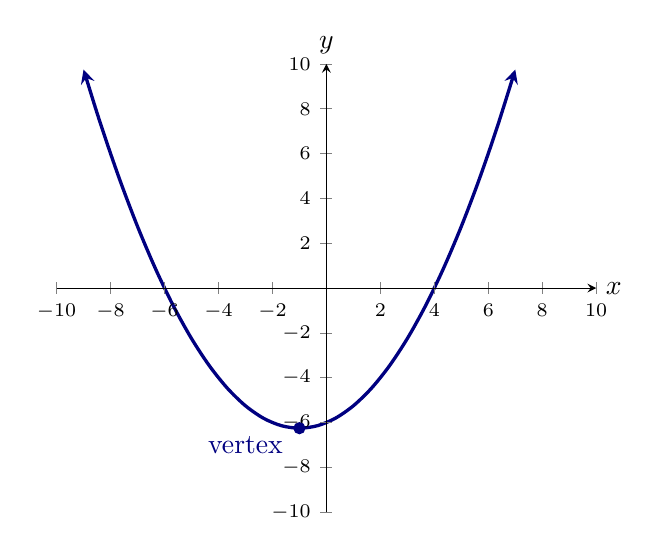
\begin{tikzpicture}
     \begin{axis}[
                domain=-10:10, ymax=10, xmax=10, ymin=-10, xmin=-10,
                axis lines =center, xlabel=$x$, ylabel=$y$,
                ytick={-10,-8,-6,-4,-2,2,4,6,8,10},
            	xtick={-10,-8,-6,-4,-2,2,4,6,8,10},
            	ticklabel style={font=\scriptsize},
                every axis y label/.style={at=(current axis.above origin),anchor=south},
                every axis x label/.style={at=(current axis.right of origin),anchor=west},
                axis on top,
                ]



        \addplot [draw=penColor, very thick, smooth, domain=(-9:7),<->] {0.25*(x+6)*(x-4)};
        %\addplot [line width=1, gray, dashed,samples=100,domain=(-9.5:9.5)] ({3},{x});
        


        \addplot [color=penColor,only marks,mark=*] coordinates{(-1,-6.25)};
        \node[penColor] at (axis cs:-3,-7) {vertex};
        %\node[penColor] at (axis cs:4,1.5) {$(h, k)$};
        %\node[penColor] at (axis cs:5,-9) {$-0.5 x^2 - 5 x + 15.5$};



    \end{axis}
\end{tikzpicture}
\end{image}










The extreme point on a parabola is called the \textbf{vertex}.  It is the lowest or highest point on the parabola, depending on whether the parabola opens up or down. 

This can be seen from the vertex form of the formula.




\[
V(x) = A \, (x - h)^2 + k
\]

The squared term, $A \, (x - h)^2$ has the same sign as $A$, except when it equals $0$.  That happens at $h$.  When $x = h$, then $V(h) = k$, which is either the minimum or maximum value of $V$.  The vertex is the graphical representation of the the extreme value of the quadratic function and where this extrema occurs in the domain.


In addition, the intercepts represent the zeros of the quadratic function and we have seen there can be $0$, $1$, or $2$ real zeros for a quadratic function.  Therefore, there can be $0$, $1$, or $2$ intercepts for a parabola.











\begin{image}
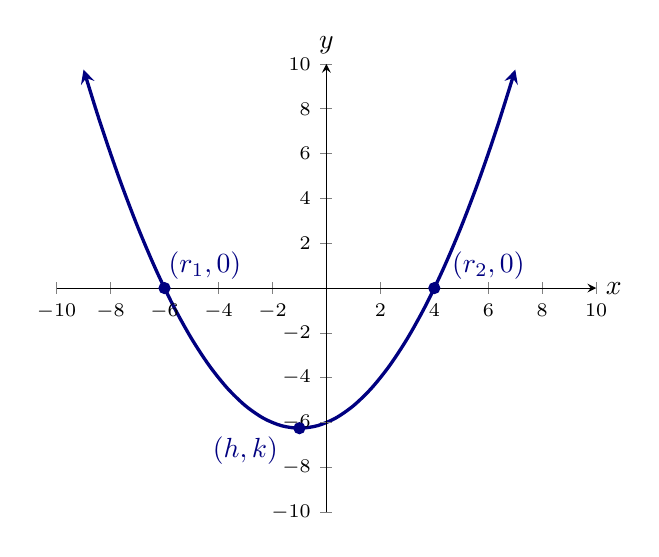
\begin{tikzpicture}
     \begin{axis}[
                domain=-10:10, ymax=10, xmax=10, ymin=-10, xmin=-10,
                axis lines =center, xlabel=$x$, ylabel=$y$,
                ytick={-10,-8,-6,-4,-2,2,4,6,8,10},
            	xtick={-10,-8,-6,-4,-2,2,4,6,8,10},
            	ticklabel style={font=\scriptsize},
                every axis y label/.style={at=(current axis.above origin),anchor=south},
                every axis x label/.style={at=(current axis.right of origin),anchor=west},
                axis on top,
                ]



        \addplot [draw=penColor, very thick, smooth, domain=(-9:7),<->] {0.25*(x+6)*(x-4)};
        %\addplot [line width=1, gray, dashed,samples=100,domain=(-9.5:9.5)] ({3},{x});
        


        \addplot [color=penColor,only marks,mark=*] coordinates{(-1,-6.25)};
        \addplot [color=penColor,only marks,mark=*] coordinates{(-6,0)};
        \addplot [color=penColor,only marks,mark=*] coordinates{(4,0)};

        \node[penColor] at (axis cs:-3,-7.25) {$(h, k)$};
        \node[penColor] at (axis cs:-4.5,1) {$(r_1, 0)$};
        \node[penColor] at (axis cs:6,1) {$(r_2, 0)$};



    \end{axis}
\end{tikzpicture}
\end{image}












\begin{example}   Analyze $f(x) = x^2 + 4 \, x - 5$ with its natural domain    \\ 




\begin{explanation} Analysis \\

$f$ is a quadratic function, since it matches the standard form, $A \, x^2 + B \, x + C$. \\


et's get the other two forms.

Factored form: $f(x) = (x+5)(x-1)$. \\

Vertex form: $f(x) = (x+2)^2 - 9$ \\




\textbf{Domain}

$f$ is a quadratic function, therefore its domain is $(-\infty, \infty)$. \\



\textbf{Zeros}

From the factored form, we can see that $-5$ and $1$ are the zeros of $f(x)$.  \\


\textbf{Continuity}

$f$ is a quadratic function, therefore it is continuous. Quadratic functions donot have singularities.\\



\textbf{End-Behavior}

$f$ is a quadratic function, with a positive leading coefficient. Therefore, its end-behavior is unbounded positively in both directions. \\

\[
\lim\limits_{x \to -\infty} f(x) = \infty 
\]


\[
\lim\limits_{x \to \infty} f(x) = \infty 
\]




\textbf{Behavior}

$f$ is a quadratic function, with a positive leading coefficient. Therefore, it will decreas and then increase. It switches behavior at the domain number for the vertex, which is


\[
-\frac{b}{2a} = -\frac{4}{2(1)} = -2
\]


$f$ decreases on $(-\infty, -2)$ and increases on $(-2, \infty )$. \\




\textbf{Maximum and Minimum}


Since $f$ decreases on $(-\infty, -2)$ and increases on $(-2, \infty )$, we have a global minimum at $-2$.   The minimum value is $f(-2) = -9$. This is also a local minimum and is the only local extrema.\\


$\lim\limits_{x \to -\infty} f(x) = \infty$ tells us that there is no global maximum. \\




\textbf{Range}

$f$ is continuous, with a global maximum and unbounded positively. \\

The range is $[-9, \infty)$. \\



\textbf{\textcolor{purple!85!blue}{A Nice Graph}}

$f$ is a quadratic function and will have a parabola for a graph.


From any of the three forms, we can see that the leading coefficient is $1$, which is positive.  Thus, our parabola will open up.


From the factored form, we can see that $-5$ and $1$ are the zeros of $f(x)$.  These will be represented by the intercepts $(-5, 0)$ and $(1,0)$.



From the vertex form, we can see that the lowest point of the parabola will be $(-2, 9)$.  Or, the function $f$ has a global minimum value of $-9$, which occurs at $-2$ in the domain.









\begin{image}
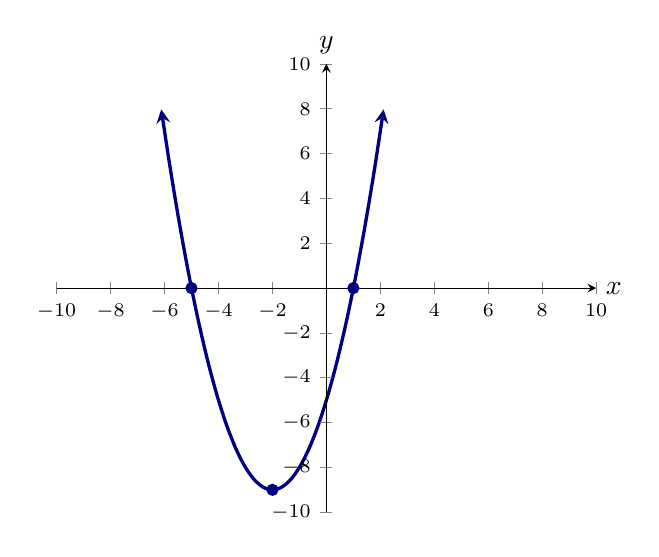
\begin{tikzpicture}
     \begin{axis}[
                domain=-10:10, ymax=10, xmax=10, ymin=-10, xmin=-10,
                axis lines =center, xlabel=$x$, ylabel=$y$,
                ytick={-10,-8,-6,-4,-2,2,4,6,8,10},
            	xtick={-10,-8,-6,-4,-2,2,4,6,8,10},
            	ticklabel style={font=\scriptsize},
                every axis y label/.style={at=(current axis.above origin),anchor=south},
                every axis x label/.style={at=(current axis.right of origin),anchor=west},
                axis on top,
                ]



        \addplot [draw=penColor, very thick, smooth, domain=(-6.12:2.12),<->] {(x+5)*(x-1)};
        %\addplot [line width=1, gray, dashed,samples=100,domain=(-9.5:9.5)] ({3},{x});
        


        \addplot [color=penColor,only marks,mark=*] coordinates{(-2,-9)};
        \addplot [color=penColor,only marks,mark=*] coordinates{(-5,0)};
        \addplot [color=penColor,only marks,mark=*] coordinates{(1,0)};




    \end{axis}
\end{tikzpicture}
\end{image}




\end{explanation}

\end{example}

















\begin{center}
\textbf{\textcolor{green!50!black}{ooooo-=-=-=-ooOoo-=-=-=-ooooo}} \\

more examples can be found by following this link\\ \link[More Examples of Quadratics]{https://ximera.osu.edu/csccmathematics/precalculus1/precalculus1/projectileMotion/examples/exampleList}

\end{center}


  



\end{document}
